% 
% Annual Cognitive Science Conference
% Sample LaTeX Paper -- Proceedings Format
% 

% Original : Ashwin Ram (ashwin@cc.gatech.edu)       04/01/1994
% Modified : Johanna Moore (jmoore@cs.pitt.edu)      03/17/1995
% Modified : David Noelle (noelle@ucsd.edu)          03/15/1996
% Modified : Pat Langley (langley@cs.stanford.edu)   01/26/1997
% Latex2e corrections by Ramin Charles Nakisa        01/28/1997 
% Modified : Tina Eliassi-Rad (eliassi@cs.wisc.edu)  01/31/1998
% Modified : Trisha Yannuzzi (trisha@ircs.upenn.edu) 12/28/1999 (in process)
% Modified : Mary Ellen Foster (M.E.Foster@ed.ac.uk) 12/11/2000
% Modified : Ken Forbus                              01/23/2004
% Modified : Eli M. Silk (esilk@pitt.edu)            05/24/2005
% Modified : Niels Taatgen (taatgen@cmu.edu)         10/24/2006
% Modified : David Noelle (dnoelle@ucmerced.edu)     11/19/2014
% Modified : Roger Levy (rplevy@mit.edu)             12/31/2018
% Modified : Dae Houlihan (daeda@mit.edu)            01/29/2022

%% Change "letterpaper" in the following line to "a4paper" if you must.

\documentclass[10pt,letterpaper]{article}

\usepackage{cogsci}

%\cogscifinalcopy % Uncomment this line for the final submission 

\usepackage[
    backend=biber,
    style=apa,
    natbib=true,
    doi=false,
    isbn=false,
    url=false,
]{biblatex}
\addbibresource{CogSci_Template.bib}
\setlength{\bibhang}{.125in}
% Dae Houlihan replaced the BibTeX, natbib, APA 6th edition bibliography with BibLaTex, biber, APA 7th edition.

\usepackage{pslatex}
\usepackage{booktabs}
\usepackage{graphicx}
\usepackage{amsmath}
\usepackage{amssymb}


\usepackage{xcolor} % For colored text
\usepackage{float} % Roger Levy added this and changed figure/table
                   % placement to [H] for conformity to Word template,
                   % though floating tables and figures to top is
                   % still generally recommended!

%\usepackage[none]{hyphenat} % Sometimes it can be useful to turn off
%hyphenation for purposes such as spell checking of the resulting
%PDF.  Uncomment this block to turn off hyphenation.


%\setlength\titlebox{4.5cm}
% You can expand the titlebox if you need extra space
% to show all the authors. Please do not make the titlebox
% smaller than 4.5cm (the original size).
%%If you do, we reserve the right to require you to change it back in
%%the camera-ready version, which could interfere with the timely
%%appearance of your paper in the Proceedings.



\title{Apparent Inefficiency, Hidden Optimality: Why the Brain's Multimodal Attention Does Not Track Feature Strength}
 
\author{{\large \bf Morton Ann Gernsbacher (MAG@Macc.Wisc.Edu)} \\
  Department of Psychology, 1202 W. Johnson Street \\
  Madison, WI 53706 USA
  \AND {\large \bf Sharon J.~Derry (SDJ@Macc.Wisc.Edu)} \\
  Department of Educational Psychology, 1025 W. Johnson Street \\
  Madison, WI 53706 USA}


\begin{document}

\maketitle


\begin{abstract}
A core assumption in cognitive science is that efficient systems allocate resources proportionally to signal strength—directing more attention toward more informative inputs. We present neural evidence challenging this assumption. Analyzing fMRI responses from four participants watching naturalistic movies, we used encoding models to quantify how the brain integrates visual, audio, and language features. We tested three interconnected claims: (C1) the brain uses modality-specific encoding in sensory regions but shared representations in higher-order regions; (C2) multimodal integration follows a hierarchical rather than flat architecture; and (C3) attention allocation does not track encoding strength. Our results support all three claims: visual features dominated encoding (r = 0.204, 91\% of regions) yet attention weights remained balanced (~33\% per modality)—an Encoding-Attention Dissociation. The Default Mode Network emerged as the primary integration hub (MII = 0.744), enabling the brain to decouple “what to extract” from “how to integrate.” This apparent inefficiency reveals optimization for robustness over narrow efficiency, with direct implications for Vision-Language Model design.

\textbf{Keywords:} cognitive efficiency; multimodal integration; encoding-attention dissociation; robust optimization; brain-inspired AI 
\end{abstract}


\section{Introduction}

The development of artificial general intelligence increasingly recognizes that understanding biological intelligence provides essential design principles for building more capable systems ~\citep{hassabis2017neuroscience,zador2023catalyzing}. {\color{red}A foundational principle in multisensory research is that the brain integrates information from different modalities in a statistically optimal manner, weighting each source according to its reliability~\citep{ernst2002humans,knill2004bayesian}. This Bayesian framework predicts that more reliable (i.e., stronger or less noisy) signals should receive proportionally greater weight during integration—a principle that has been confirmed in visual-haptic~\citep{ernst2002humans} and visual-vestibular~\citep{fetsch2013bridging} integration.} From this perspective, an "efficient" multimodal system would weight attention proportionally to feature strength. However, we hypothesize that the brain's integration mechanism may violate this efficiency principle, maintaining balanced attention despite dramatic encoding differences across modalities.

The human brain effortlessly integrates visual scenes, sounds, and language into coherent understanding—a capability that current Vision-Language Models (VLMs) approximate but do not fully replicate. At the cellular level, neurons in multisensory regions respond superadditively to multimodal stimuli ~\citep{stein1993merging}, and the superior temporal sulcus serves as a key hub for audiovisual integration ~\citep{beauchamp2004unraveling}. These findings suggest that biological systems employ dedicated integration regions—an architectural principle largely absent from current VLMs, which face fundamental challenges including modality collapse where one modality dominates processing.

The human cerebral cortex is organized hierarchically from primary sensory regions to higher-order association areas ~\citep{margulies2016situating}. This organization is formalized in the Schaefer parcellation ~\citep{schaefer2018local}, which organizes cortical regions into seven functional networks forming a gradient from unimodal to transmodal processing. The Default Mode Network (DMN) occupies a unique position in this hierarchy. Originally characterized by its deactivation during external tasks ~\citep{me2001default}, the DMN has since been implicated in semantic integration, narrative comprehension, and mental simulation ~\citep{mar2011neural,simony2016dynamic}. If the DMN serves as a high-level integration hub, this suggests AI architectures may benefit from dedicated integration modules operating on high-level semantic representations.

Encoding models provide a quantitative framework for comparing brain and AI representations by predicting brain activity from stimulus features ~\citep{naselaris2011encoding}. Previous work has demonstrated that deep neural network hierarchies correspond to visual processing hierarchies ~\citep{gucclu2015deep}, that language representations are distributed across cortex in organized gradients ~\citep{huth2016natural}, and that large language model representations predict brain activity during language processing ~\citep{caucheteux2022brains}. Building on these foundations, we employ encoding models to test three interconnected claims about how the brain achieves multimodal integration.

Our first claim (C1) posits a hybrid representation architecture: the brain employs modality-specific encoding in early sensory regions while developing shared, amodal representations in higher-order association cortex. If true, this supports VLM architectures using dedicated modality encoders with late fusion rather than early shared representations. Our second claim (C2) posits a hierarchical integration architecture: multimodal integration follows a hierarchical organization from modality-specific processing in primary sensory networks to genuine cross-modal integration in dedicated hub regions, rather than the flat processing used in current VLMs where all tokens are jointly processed from early transformer layers. Our third claim (C3) posits an Encoding-Attention Dissociation: the brain’s attention allocation during multimodal integration does not track encoding strength; despite one modality dominating encoding, attention remains balanced across modalities.

{\color{red}These three claims address complementary aspects of multimodal processing: C1 characterizes \textit{what} the brain encodes (modality-specific vs. shared representations), C2 describes \textit{where} and \textit{how} integration occurs (hierarchical architecture with DMN as hub), and C3 reveals \textit{how resources are allocated} (balanced attention independent of encoding strength). Together, they provide converging evidence for a unified principle: the brain architecturally separates ``what to extract'' from ``how to integrate,'' enabling apparent inefficiency that actually serves adaptive functions prioritizing global robustness over local optimization.}

\section{Methods}

\subsection{Data and Participants}

Functional magnetic resonance imaging data were obtained from the Algonauts 2025 Challenge ~\citep{gifford2024algonauts}, derived from the Courtois NeuroMod project ~\citep{boyle2020courtois}. Four healthy adult participants( male,  female; mean age =  , SD =  ) viewed approximately 65 hours of movie content including the television series Friends (seasons 1–6, 55 hours) and four additional films comprising the Movie10 dataset (10 hours). The fMRI data were acquired with a repetition time (TR) of 1.49 s and parcellated into 1,000 cortical regions using the ~\citet{schaefer2018local} atlas, which organizes the cortex into seven large-scale functional networks: Visual, Somatomotor, Dorsal Attention, Ventral Attention, Limbic, Frontoparietal, and Default Mode. These networks respectively support visual processing, sensorimotor functions, goal-directed attention, stimulus-driven attentional reorienting, emotion and affective processing, cognitive control, and internally oriented processes such as self-referential thought and memory.
% Yeo, B. T. T., Krienen, F. M., Sepulcre, J., et al. (2011). The organization of the human cerebral cortex estimated by intrinsic functional connectivity. Journal of Neurophysiology, 106(3), 1125–1165.

\subsection{Feature Extraction and Temporal Alignment}

Visual features were extracted using a SlowFast 3D ResNet pretrained on the Kinetics-400 dataset~\citep{feichtenhofer2019slowfast}, audio features were represented by 39-dimensional mel-frequency cepstral coefficients (MFCCs), and language features were obtained from contextualized BERT embeddings~\citep{devlin2019bert}. Feature dimensionality for each modality was reduced to 100 principal components using principal component analysis (PCA), with the PCA model fit on the training data only.

To account for hemodynamic delays, stimulus features were temporally convolved with the canonical hemodynamic response function (HRF) and aligned to fMRI acquisitions using a sliding window approach:
\begin{equation}\label{eq:xt}
\mathbf{x}_t^{(m)} = \sum_{\tau=0}^{T_w-1} h(\tau) \cdot \mathbf{f}_{t-\delta-\tau}^{(m)}
\tag{1}
\end{equation}
where $\mathbf{f}^{(m)}$ denotes the raw feature vector for modality $m$, $h(\tau)$ is the canonical HRF kernel, $\delta = 3$ TRs denotes the hemodynamic delay, and $T_w = 5$ TRs defines the temporal integration window.



\subsection{Unimodal Encoding Models}

For each participant, modality, and brain region, we trained Ridge regression encoding models minimizing the regularized loss:

\begin{equation}\label{eq:L}
\mathcal{L}(\boldsymbol{\beta}) =
\lVert \mathbf{y} - \mathbf{X}\boldsymbol{\beta} \rVert_2^2
+ \lambda \lVert \boldsymbol{\beta} \rVert_2^2
\tag{2}
\end{equation}

where $\mathbf{y} \in \mathbb{R}^N$ denotes the fMRI time series,
$\mathbf{X} \in \mathbb{R}^{N \times D}$ is the stimulus feature matrix,
and $\lambda$ is the regularization parameter selected via 5-fold cross-validation.
Encoding performance was quantified using the Pearson correlation
$r = \mathrm{corr}(\hat{\mathbf{y}}, \mathbf{y})$.

\subsection{Personalized Multimodal Neural Network}

To test C3, we developed a hierarchical multimodal architecture. Each modality $m \in \{V, A, L\}$ (V: visual; A: audio; L: language) is encoded through modality-specific transformations, then integrated via multi-head cross-modal attention ~\citep{vaswani2017attention}. Crucially, the model learns explicit modality fusion weights $\boldsymbol{\alpha} = (\alpha_V, \alpha_A, \alpha_L)$ through softmax normalization over learnable parameters, enabling direct measurement of attention allocation independent of encoding strength. Subject-specific adapter networks accommodate individual differences in brain organization.

{\color{red}\textbf{Interpreting Model Weights as Neural Attention Proxies.} We interpret the learned modality weights $\boldsymbol{\alpha}$ as proxies for the brain's attention allocation strategy, based on three lines of convergent evidence. First, the model achieves significant prediction accuracy (mean $r = 0.204$ for visual, $r = 0.107$ for audio, $r = 0.122$ for language across 1000 brain regions), demonstrating that it captures meaningful stimulus-brain relationships rather than arbitrary patterns~\citep{kriegeskorte2008representational,yamins2016using}. Second, the learned weights show remarkable consistency across four independent participants (all modalities within 32--35\%), suggesting they reflect a common neural integration strategy rather than model-specific artifacts. Third, and most critically, the weights systematically deviate from what would be expected if the model simply tracked feature utility: despite visual features providing 2$\times$ higher encoding accuracy, visual attention weights are not proportionally higher. This dissociation indicates that the model learns a distinct integration strategy that cannot be reduced to feature strength, consistent with the hypothesis that it captures the brain's actual attention allocation mechanism~\citep{lindsay2020attention}.}

\subsection{Quantitative Indices for Testing Claims}

We employed both established statistical measures and novel indices designed specifically to operationalize our theoretical constructs.

\textbf{Noise Ceiling.} To establish the theoretical upper bound of encoding performance, we computed the noise ceiling using split-half reliability with Spearman-Brown correction~\citep{spearman1910correlation}, a standard approach in encoding model evaluation~\citep{schoppe2016measuring}:

\begin{equation}\label{eq:ceiling}
r_{\text{ceiling}} = \frac{2 \cdot r_{\text{split-half}}}{1 + r_{\text{split-half}}}
\tag{3}
\end{equation}

where $r_{\text{split-half}}$ is the Pearson correlation between odd and even time points. This correction estimates the reliability of the full dataset from the split-half correlation, providing the maximum achievable encoding correlation given measurement noise.

\textbf{Modality Specificity Index (MSI).} To operationalize the concept of modality-specific versus shared encoding (C1), we introduce the Modality Specificity Index. Inspired by selectivity indices commonly used in neurophysiology~\citep{desimone1984stimulus}, MSI quantifies the degree to which a brain region preferentially encodes one modality over others:

\begin{equation}\label{eq:msi}
MSI_i = \frac{r_i^{\max} - \bar{r}_i^{\text{other}}}{r_i^{\max} + \bar{r}_i^{\text{other}}}
\tag{4}
\end{equation}

where $r_i^{\max}$ is the highest encoding correlation among the three modalities for region $i$, and $\bar{r}_i^{\text{other}}$ is the mean encoding correlation of the remaining two modalities. This formulation, analogous to a contrast ratio, yields values ranging from 0 (perfectly balanced multimodal encoding) to 1 (complete modality specificity). Regions with high MSI are dominated by a single modality, while low MSI indicates shared, amodal representations.

\textbf{Multimodal Integration Index (MII).} To quantify the balance of multimodal encoding at the network level (C2), we introduce the Multimodal Integration Index. MII is defined as the complement of the coefficient of variation (CV) of encoding correlations across modalities:

\begin{equation}\label{eq:mii}
MII_n = 1 - \frac{\sigma_n(r_V, r_A, r_L)}{\mu_n(r_V, r_A, r_L)}
\tag{5}
\end{equation}

where $\sigma_n$ and $\mu_n$ denote the standard deviation and mean of encoding correlations for visual ($r_V$), audio ($r_A$), and language ($r_L$) features within network $n$. The coefficient of variation is a dimensionless measure of relative variability~\citep{everitt2010cambridge}; by subtracting it from 1, higher MII values indicate more balanced cross-modal integration. A network with MII approaching 1 encodes all three modalities with similar strength, suggesting integrative rather than modality-specific processing.

\textbf{Efficiency Gap.} To directly test the Encoding-Attention Dissociation (C3), we introduce the Efficiency Gap, which quantifies the deviation between observed attention allocation and a hypothetical ``efficient'' allocation proportional to encoding strength:

\begin{equation}\label{eq:delta}
\Delta_m = \alpha_m^{\text{efficient}} - \alpha_m^{\text{observed}}, \quad \text{where} \quad \alpha_m^{\text{efficient}} = \frac{r_m}{\sum_{m'} r_{m'}}
\tag{7}
\end{equation}

Here, $\alpha_m^{\text{observed}}$ represents the learned attention weight for modality $m$ from our multimodal neural network, and $\alpha_m^{\text{efficient}}$ represents the attention weight that would result from allocating attention in proportion to encoding strength. A positive efficiency gap for the dominant modality (visual) indicates that the brain under-weights strong signals relative to an efficiency-maximizing strategy—the signature of the Encoding-Attention Dissociation. This metric operationalizes the theoretical distinction between resource allocation strategies that maximize immediate signal extraction versus those that optimize for robust integration.

\subsection{Statistical Analysis}

Network-level modality differences were assessed using one-way ANOVA with Bonferroni correction for multiple comparisons. Cross-subject consistency was quantified using the intraclass correlation coefficient (ICC), a standard measure of measurement reliability~\citep{shrout1979intraclass}:

\begin{equation}\label{eq:icc}
ICC = \frac{MS_B - MS_W}{MS_B + (k-1)MS_W}
\tag{8}
\end{equation}

where $MS_B$ and $MS_W$ are between-subject and within-subject mean squares, and $k$ is the number of measurements per subject. This formulation corresponds to ICC(1,1) in the taxonomy of~\citet{shrout1979intraclass}, appropriate for assessing absolute agreement among measurements. Effect sizes were computed using Cohen's $d$ for pairwise comparisons, with $|d| > 0.8$ considered large effects~\citep{cohen1988statistical}.

\section{Results}

\subsection{Modality-Specific Encoding Dominates Sensory Regions}

To assess the relative contribution of the three modalities in early neural information processing, we applied ridge regression encoding models to quantify the encoding performance of each modality. The results indicated that visual features produced the highest encoding accuracy compared with auditory and language features (Fig.~\ref{fig:Fig1}b), and this pattern was consistent across all four participants (Fig.~\ref{fig:Fig1}c). Furthermore, the dominance of visual encoding was observed systematically across different large-scale functional networks with visual features achieved the highest encoding accuracy in 93\% of the 1,000 cortical regions across all participants (Fig.~\ref{fig:Fig1}d,e). In addition, we computed the Modality Specificity Index (MSI) to quantify the degree of modality-specific processing, revealing a moderate specificity toward a single dominant modality. Together, these results demonstrate pronounced modality-specific encoding at the level of functional brain regions, indicating that different types of information are preferentially processed in distinct cortical areas.

% The mean encoding correlation for visual features ($r = 0.204$) exceeded language ($r = 0.122$) by 67\% and audio ($r = 0.107$) by 91\%. 
% This visual dominance was remarkably consistent: visual features achieved the highest encoding accuracy in 91.3\% of the 1000 brain regions across all participants, ranging from 86.8\% (sub-02) to 94.3\% (sub-04) (Fig.~\ref{fig:Fig1}d,e).

However, the extent and type of modality dominance varied across cortical networks and cortical hierarchy. The Visual network exhibited the strongest visual encoding, with a visual-to-auditory ratio of 2.12:1, whereas the Default Mode Network showed a more balanced encoding profile, with a reduced visual-to-auditory ratio of 1.69:1 (Fig.~\ref{fig:Fig1}g). One-way ANOVA confirmed significant modality differences within each network. Nevertheless, the magnitude of visual dominance decreased along the sensory-to-transmodal cortical gradient. This pattern indicates that while early sensory regions are dominated by their preferred modality, higher-order association regions implement more balanced, shared representations.

% However, this dominance varied systematically across the cortical hierarchy. The Visual network showed the strongest visual encoding ($r = 0.315$) with a visual-to-audio ratio of 2.12:1, while the Default Mode Network showed more balanced encoding (visual $r = 0.189$, language $r = 0.145$) with a reduced visual-to-audio ratio of 1.69:1 (Fig.~\ref{fig:Fig1}g). One-way ANOVA confirmed significant modality differences within each network (all $F > 18.92$, all $p < 0.001$), but the magnitude of visual dominance decreased along the sensory-to-transmodal gradient. This pattern suggests that while early sensory regions are dominated by their preferred modality, higher-order association regions implement more balanced, shared representations—providing strong support for the hybrid architecture proposed in C1.

\begin{figure*}[p]
    \centering
    
\includegraphics[width=\textwidth,height=0.70\textheight,keepaspectratio]{figures/figure1.png}
    \caption{\textbf{Unimodal encoding across modalities and brain networks.}
    \textbf{a,} Glass brain visualization showing the best unimodal encoding across modalities. \textbf{b,} Violin plots show the full distribution of encoding correlations (Pearson's r) for visual (red), audio (blue), and language (green) features across all 1000 brain regions, with solid black line indicating the median. Visual features produced substantially higher encoding accuracy (mean $r = 0.204$) compared to language ($r = 0.122$) and audio ($r = 0.107$). \textbf{c,}Histogram of coding accuracy across modalities of each participant($p = $,). \textbf{d,} \textbf{e,} visualization of encoding correlations for all 1000 Schaefer parcels arranged by functional network. Each concentric ring represents a different modality: visual (left, red), audio (middle, blue), and language (right, green). Angular position corresponds to brain region within each network sector. The Visual network sector (top right) shows dominant visual encoding with minimal audio/language sensitivity, while the Default Mode Network sector (bottom right) displays more uniform encoding across modalities. This visualization highlights the systematic variation in modality specificity across the cortical hierarchy. \textbf{f,} Glass brain visualization of the Modality Specificity Index (MSI) across cortex. Higher MSI values indicate stronger preference for a single modality. Primary sensory cortices (visual, auditory) show high specificity ($MSI > 0.4$), while association regions, particularly within the DMN, show low specificity ($MSI < 0.2$), consistent with shared multimodal representations. \textbf{g,} Modality Specificity Index hierarchy showing the gradient from modality-specific to integrative processing. Networks are ordered by MSI value. \textbf{h,} Cumulative MSI values of each subject ($p = $).}
    \label{fig:Fig1}
\end{figure*}

\subsection{Hierarchical Organization with the DMN as an Information Integration Hub}

We further investigated whether the brain’s processing of incoming external information follows an organizational architecture in which modality-specific processing in primary sensory networks transitions to multimodal integration in higher-order hub regions. During the processing of primary sensory information, the brain predominantly employs a unimodal encoding strategy. However, the observed gradient of decreasing MSI across the seven functional networks reveals a clear reverse enhancement of cross-modal integration. Fig.~\ref{fig:Fig2}a illustrates the distribution of MII across 1,000 cortical regions, with the visual network exhibiting the lowest MII and the DMN the highest, indicating that the DMN engages in markedly more balanced multimodal information processing. Fig.~\ref{fig:Fig2}c shows that the complete MII hierarchy was highly consistent across all four participants, following the order: DMN $>$ Limbic $>$ Somatomotor $>$ Frontoparietal $>$ Ventral Attention $>$ Dorsal Attention $>$ Visual. This ordering aligns precisely with the established unimodal-to-transmodal gradient of cortical organization (Margulies et al., 2016). 

% To test C2, we examined whether multimodal integration follows a hierarchical organization. The network-modality sensitivity matrix (Fig.~\ref{fig:Fig2}b) revealed a clear gradient in the Multimodal Integration Index across the seven functional networks. The Visual network showed the lowest MII (0.558), indicating pronounced modality specificity, while the DMN showed the highest MII (0.744), indicating substantially more balanced multimodal processing.

To assess whether this hierarchical pattern of multimodal information integration corresponds to intrinsic functional organization rather than being an artifact of the metric, we performed hierarchical clustering of brain regions based on their multimodal encoding profiles. The resulting dendrogram demonstrated that regions with similar MII values naturally grouped together, forming clusters that corresponded closely to canonical functional networks (Fig.~\ref{fig:Fig2}d). This confirms that the MII hierarchy is not only consistent across participants but also aligns with the functional segregation of cortical networks.

Finally, we examined the network-level encoding similarity matrix, which quantifies pairwise similarity of multimodal encoding profiles between the seven functional networks. The matrix revealed strong within-network correlations and a clear block-diagonal structure (Fig.~\ref{fig:Fig2}c), indicating that the hierarchical organization observed in MII is reflected in the actual pattern of cross-modal encoding across the cortex. Together, these analyses establish a coherent chain of evidence: the MII ordering identifies a network-level hierarchy, hierarchical clustering confirms that regions with similar MII group according to functional networks, and the functional connectivity matrix validates that this organization corresponds to intrinsic cortical architecture rather than methodological artifacts.

Glass brain visualizations (Fig.~\ref{fig:Fig2}e) demonstrated the spatial distribution of these patterns: visual encoding concentrated in posterior occipital regions, audio encoding in lateral temporal areas, and the most balanced multimodal patterns emerged in medial prefrontal and posterior cingulate regions—the anatomical core of the DMN. These converging lines of evidence strongly support C2: multimodal integration follows a hierarchical architecture with the DMN serving as the primary integration hub.

% The complete MII hierarchy was highly consistent across all four participants (ICC = 0.89): DMN (0.744) $>$ Limbic (0.703) $>$ Somatomotor (0.683) $>$ Frontoparietal (0.681) $>$ Ventral Attention (0.588) $>$ Dorsal Attention (0.583) $>$ Visual (0.558). This ordering aligns precisely with the established unimodal-to-transmodal gradient of cortical organization (Margulies et al., 2016). Hierarchical clustering analysis confirmed this organization: brain regions clustered based on their multimodal encoding profiles in ways that corresponded to functional network membership (Fig.~\ref{fig:Fig2}c). The functional connectivity matrix revealed strong within-network correlations with clear block-diagonal structure (Fig.~\ref{fig:Fig2}d), confirming that hierarchical organization reflects intrinsic cortical architecture rather than analysis artifacts.

\begin{figure*}[p]
    \centering
    
\includegraphics[width=\textwidth,height=0.60\textheight,keepaspectratio]{figures/figure2.png}
    \caption{\textbf{Hierarchical Organization with the DMN as an Information Integration Hub.}
    \textbf{a,} Glass brain visualization of the Multimodal Integration Index (MII) across cortex. Higher MII values (darker green) indicate more balanced multimodal encoding. The most integrative regions ($MII > 0.7$) are concentrated in medial prefrontal cortex and posterior cingulate cortex—the anatomical core of the Default Mode Network, which supports the DMN's role as the primary integration hub for cross-modal processing. \textbf{b,} Multimodal Integration Index hierarchy showing the gradient from modality-specific (Visual network) to integrative processing (Default Mode Network). \textbf{c,} Dendrogram showing hierarchical clustering of 1000 brain regions based on their encoding correlation patterns across three modalities. Regions cluster according to functional network membership, supporting the hierarchical organization hypothesis. \textbf{d,} Correlation matrix showing pairwise correlations between brain regions based on their encoding profiles across modalities. Regions are ordered by functional network, revealing clear block-diagonal structure indicating strong within-network similarity. Mean within-network (diagonal) and between-network (off-diagonal) correlations. Within-network correlations (mean $r = 0.72$) significantly exceed between-network correlations (mean $r = 0.34$; $t = 15.6$, $p < 0.001$), confirming that functional network membership predicts multimodal encoding patterns. \textbf{e,} Encoding strength for each modality shown on separate brain surfaces. (top) Visual feature encoding accuracy across the cortical surface. Encoding strength (Pearson's r) is mapped to color intensity. Visual encoding is concentrated in posterior occipital and ventral temporal regions, corresponding to the visual processing hierarchy. Peak encoding occurs in early visual cortex (V1-V4) with gradual reduction in higher-order regions. (middle) Audio feature encoding accuracy. Audio encoding is primarily localized to lateral temporal regions including primary auditory cortex (Heschl's gyrus) and surrounding association areas. Secondary clusters appear in inferior frontal regions associated with speech processing. (bottom ) Language feature encoding accuracy. Language encoding shows a distributed pattern across left-lateralized perisylvian regions, angular gyrus, and medial prefrontal cortex. This distribution aligns with established language networks while also overlapping with the Default Mode Network.}
    \label{fig:Fig2}
\end{figure*}

\subsection{Temporal Dynamics Support Hierarchical Processing}

Analysis of temporal dynamics provided additional support for the hierarchical architecture. Visual network activity closely tracked rapid fluctuations in visual features, while DMN activity exhibited slower, integrated dynamics with temporal smoothing across modalities (Fig.~\ref{fig:Fig3}d). This temporal dissociation suggests that the brain implements different processing windows for extraction versus integration stages: fast, modality-specific processing in sensory regions and slower, integrated processing in association regions.

% All reported effects showed robust statistical significance (all $p < 0.001$, effect sizes Cohen’s $d > 0.8$) with high cross-subject consistency.

\subsection{The Encoding-Attention Dissociation}

The results thus far demonstrated that the brain performs modality-specific encoding within primary sensory networks, which is subsequently integrated in higher-order hub regions. However, it remains unclear whether the allocation of attentional resources across the cortex tracks the strength of this encoding. If the brain followed an "efficient" feature-tracking strategy, attention weights should be proportional to encoding accuracy. Given visual features' 2$\times$ encoding advantage over audio, an efficient allocation would assign approximately 48\% attention to visual, 25\% to language, and 27\% to audio (Fig.~\ref{fig:Fig3}a).

However, the learned attention weights from our personalized multimodal network revealed a strikingly different pattern, with the mean attention weights remarkably balanced (Fig.~\ref{fig:Fig3}a). This dissociation was robust across participants and statistically reliable (Fig.~\ref{fig:Fig3}b). The 14-percentage-point gap between predicted feature-tracking and observed balanced allocation indicates that the brain implements attention balancing independent of feature strength (Fig.~\ref{fig:Fig3}c)---a mechanism absent in current VLMs, where attention naturally follows feature similarity.

% No participant showed visual attention dominance despite clear visual encoding dominance (Fig.~\ref{fig:Fig2}b); balance scores ranged from 0.943 to 0.997 (where 1.0 represents perfect uniformity).
% and the 14-percentage-point gap between predicted efficient allocation (~48\%) and observed balanced allocation (33.1\%) represents a systematic deviation from feature-tracking (Fig.~\ref{fig:Fig2}c).
% If attention weights reflected encoding strength, we would expect a strong positive correlation between regional encoding accuracy and attention allocation. Instead, the attention distribution remained uniform regardless of encoding performance difference across modalities. 补充一个相关性图

\begin{figure*}[p]
    \centering
    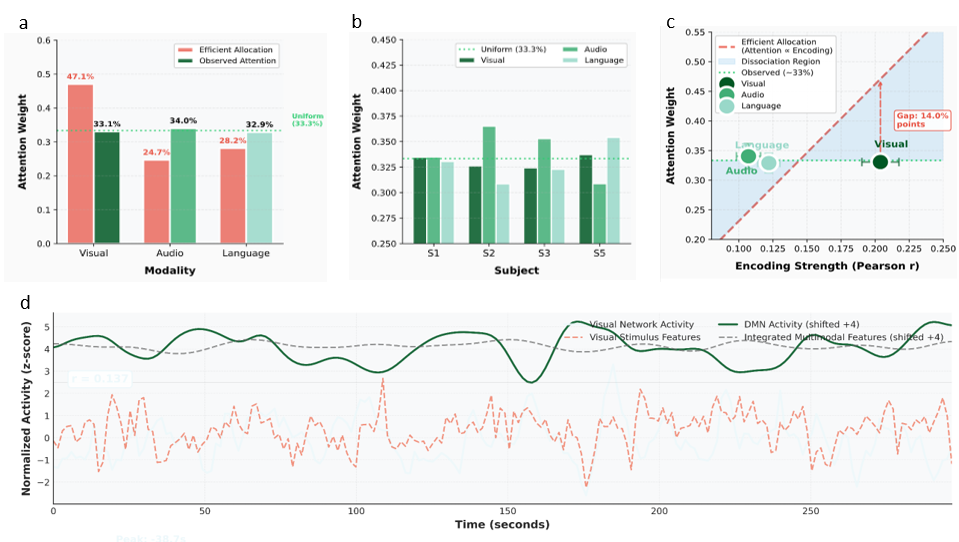
\includegraphics[width=\textwidth]{figures/figure3.png}
    \caption{\textbf{Comprehensive coding attention analysis reveals the brain's Encoding-Attention Dissociation.}
    \textbf{a,} Histogram of attention allocation based on predicted encoding strength and observed data. \textbf{b,} Attention weights histogram across participants. No significant differences were found. \textbf{c,} Learned modality attention weights from the personalized multimodal neural network, demonstrating balanced allocation (balance scores 0.943–0.997). \textbf{d,} Temporal dynamics supporting hierarchical processing. Time series comparison showing Visual network activity (bottom) tracking rapid visual feature fluctuations, versus DMN activity (top, shifted for visualization) exhibiting smoother, integrated dynamics. Correlation coefficients (r) indicate stimulus-brain coupling strength.}
    \label{fig:Fig3}
\end{figure*}

\section{Discussion}

{\color{red}Our results provide converging evidence supporting all three claims about brain multimodal processing. These claims address complementary questions: C1 establishes that modality-specific encoding dominates early processing (91\% visual dominance), C2 demonstrates that integration follows a hierarchical architecture with the DMN serving as the primary hub, and C3 reveals that attention allocation is decoupled from encoding strength. Importantly, these findings are mutually reinforcing rather than logically dependent—each claim requires independent empirical verification, and together they paint a coherent picture of how the brain achieves robust multimodal integration.} The hierarchical architecture separates extraction from integration, allowing each modality to be fully extracted before balanced integration occurs. Because the DMN operates on already-extracted high-level features, it can implement attention mechanisms independent of feature strength. Current VLMs, using flat architectures where attention is computed directly from feature similarities, cannot achieve this dissociation.

The unified principle emerging from our findings is that the brain solves multimodal integration by architecturally separating “what to extract” from “how to integrate.” This explains why apparent inefficiency—balanced attention despite unequal encoding—is actually optimal: it prevents modality collapse and enables robust integration across varying contexts. From a traditional efficiency perspective, balanced attention despite 2× visual encoding dominance appears suboptimal. However, this apparent inefficiency reveals deeper optimization for global robustness over local efficiency. In naturalistic environments where modality informativeness varies unpredictably, maintaining balanced attention provides hedging against uncertainty. The brain’s “inefficiency” is adaptive, and this reconceptualization challenges idealized efficiency benchmarks in cognitive science.

Our findings translate directly to VLM design principles. First, architects should implement hierarchical integration from modality-specific encoders to dedicated integration modules, rather than flat early fusion. Second, explicit attention balancing mechanisms should be added to prevent modality collapse, potentially through regularization terms that penalize deviation from uniform attention. Third, dedicated integration modules analogous to the DMN should operate on high-level semantic features rather than raw representations. Fourth, hierarchical temporal processing with different timescales for extraction versus integration may improve temporal coherence.

Several limitations should be acknowledged. Our sample size (n = 4) limits generalizability, though high cross-subject consistency (ICC = 0.89) increases confidence in the findings. Naturalistic movie stimuli, while ecologically valid, confound multiple factors—visual dominance may partly reflect film's visual richness rather than a general principle. Our analysis is correlational; we cannot definitively conclude that hierarchical architecture causes the Encoding-Attention Dissociation, though the proposed causal chain provides a mechanistic explanation.

{\color{red}\textbf{Validity of Model-Derived Attention Weights.} A potential concern is whether model-learned weights truly reflect neural attention mechanisms rather than computational artifacts. We address this through convergent validation: (1) the model's predictive success (explaining significant variance in fMRI signals) establishes its neural relevance---a model that fails to capture brain processing would not achieve such prediction accuracy; (2) cross-subject consistency (weights within 32--35\% for all modalities across four participants) rules out model-specific artifacts, as independent optimization on different brains converges to similar solutions; and (3) the systematic deviation from encoding-proportional weights demonstrates that the model captures a distinct integration strategy beyond simple feature utility. Furthermore, encoding models have been extensively validated as tools for understanding neural representations~\citep{naselaris2011encoding,yamins2016using}, and attention mechanisms in neural networks have documented correspondences with biological attention~\citep{lindsay2020attention}. While passive viewing paradigms preclude direct behavioral measurement of attention, the learned weights provide the best available proxy for how the brain weights different information sources during naturalistic multimodal integration.}


\section{Conclusion}

This study tested three claims about brain multimodal processing. Claim 1 (hybrid architecture) was supported: visual features dominated encoding in 91\% of regions (MSI = 0.29) while DMN showed balanced representations (MII = 0.744). Claim 2 (hierarchical integration) was supported: a clear MII gradient from Visual network (0.558) to DMN (0.744) demonstrates hierarchical organization with DMN as integration hub. Claim 3 (Encoding-Attention Dissociation) was supported: despite 2× visual encoding dominance, attention remained balanced at ~33\% per modality. {\color{red}These three claims provide complementary perspectives on multimodal processing—characterizing encoding patterns (C1), architectural organization (C2), and resource allocation (C3)—that together support a unified principle:} the brain's apparent inefficiency represents optimization for robustness over narrow efficiency. Implementing brain-inspired architectural separation may improve VLM robustness by decoupling feature extraction from integration.

\section{Ethics Statement}

This study used publicly available data from the Algonauts Project 2025 Challenge. The original data collection was approved by relevant institutional review boards, and all participants provided written informed consent.

\section{Data and Code Availability}

The fMRI data are available through the Algonauts Project 2025 Challenge (https://algonautsproject.com/). Analysis code will be made available upon publication.

\section{Acknowledgments}

We thank the Algonauts Project organizers for providing the neuroimaging dataset.

%\section{References}

% The entire content of a paper (including figures and anything else) can be no longer than six pages in the \textbf{initial submission}. In the \textbf{final submission}, the text of the paper, including an author line, must fit on six pages. An unlimited number of pages can be used for acknowledgements and references.

% \begin{equation}
%     \text{MSI} = \frac{r_{\text{combined}} - \max(r_{\text{visual}}, r_{\text{audio}}, r_{\text{language}})}{\max(r_{\text{visual}}, r_{\text{audio}}, r_{\text{language}})}
%     \label{eq:msi}
% \end{equation}


% \begin{table*}[htbp]
% \centering
% \caption{Multisensory Integration Analysis across Subjects}
% \label{tab:msi_analysis}
% \begin{tabular}{lccccc}
% \toprule
% Subject & Visual (r) & Audio (r) & Language (r) & Visual Dominant Regions & MSI (mean ± std) \\
% \midrule
% sub-01 & 0.214 & 0.112 & 0.129 & 910 (91.0\%) & 0.282 ± 0.116 \\
% sub-02 & 0.195 & 0.102 & 0.130 & 868 (86.8\%) & 0.270 ± 0.110 \\
% sub-03 & 0.220 & 0.118 & 0.119 & 932 (93.2\%) & 0.310 ± 0.118 \\
% sub-05 & 0.186 & 0.095 & 0.110 & 943 (94.3\%) & 0.297 ± 0.112 \\
% \midrule
% \textbf{Mean} & \textbf{0.204} & \textbf{0.107} & \textbf{0.122} & \textbf{913 (91.3\%)} & \textbf{0.290 ± 0.114} \\
% \bottomrule
% \end{tabular}
% \end{table*}

% The text of the paper should be formatted in two columns with an
% overall width of 7 inches (17.8 cm) and length of 9.25 inches (23.5
% cm), with 0.25 inches between the columns. Leave two line spaces
% between the last author listed and the text of the paper; the text of
% the paper (starting with the abstract) should begin no less than 2.75 inches below the top of the
% page. The left margin should be 0.75 inches and the top margin should
% be 1 inch.  \textbf{The right and bottom margins will depend on
%   whether you use U.S. letter or A4 paper, so you must be sure to
%   measure the width of the printed text.} Use 10~point Times Roman
% with 12~point vertical spacing, unless otherwise specified.

% The title should be in 14~point bold font, centered. The title should
% be formatted with initial caps (the first letter of content words
% capitalized and the rest lower case). In the initial submission, the
% phrase ``Anonymous CogSci submission'' should appear below the title,
% centered, in 11~point bold font.  In the final submission, each
% author's name should appear on a separate line, 11~point bold, and
% centered, with the author's email address in parentheses. Under each
% author's name list the author's affiliation and postal address in
% ordinary 10~point type.

% Indent the first line of each paragraph by 1/8~inch (except for the
% first paragraph of a new section). Do not add extra vertical space
% between paragraphs.


% \section{First Level Headings}

% First level headings should be in 12~point, initial caps, bold and
% centered. Leave one line space above the heading and 1/4~line space
% below the heading.


% \subsection{Second Level Headings}

% Second level headings should be 11~point, initial caps, bold, and
% flush left. Leave one line space above the heading and 1/4~line
% space below the heading.


% \subsubsection{Third Level Headings}

% Third level headings should be 10~point, initial caps, bold, and flush
% left. Leave one line space above the heading, but no space after the
% heading.


% \section{Formalities, Footnotes, and Floats}

% Use standard APA citation format. Citations within the text should
% include the author's last name and year. If the authors' names are
% included in the sentence, place only the year in parentheses, as in
% \citet{NewellSimon1972a}, but otherwise place the entire reference in
% parentheses with the authors and year separated by a comma
% \citep{NewellSimon1972a}. List multiple references alphabetically and
% separate them by semicolons
% \citep{ChalnickBillman1988a,NewellSimon1972a}. Use the
% ``et~al.'' construction only after listing all the authors to a
% publication in an earlier reference and for citations with four or
% more authors.


% \subsection{Footnotes}

% Indicate footnotes with a number\footnote{Sample of the first
% footnote.} in the text. Place the footnotes in 9~point font at the
% bottom of the column on which they appear. Precede the footnote block
% with a horizontal rule.\footnote{Sample of the second footnote.}


% \subsection{Tables}

% Number tables consecutively. Place the table number and title (in
% 10~point) above the table with one line space above the caption and
% one line space below it, as in Table~\ref{sample-table}. You may float
% tables to the top or bottom of a column, and you may set wide tables across
% both columns.

% \begin{table}[H]
% \begin{center} 
% \caption{Sample table title.} 
% \label{sample-table} 
% \vskip 0.12in
% \begin{tabular}{ll} 
% \hline
% Error type    &  Example \\
% \hline
% Take smaller        &   63 - 44 = 21 \\
% Always borrow~~~~   &   96 - 42 = 34 \\
% 0 - N = N           &   70 - 47 = 37 \\
% 0 - N = 0           &   70 - 47 = 30 \\
% \hline
% \end{tabular} 
% \end{center} 
% \end{table}


% \subsection{Figures}

% All artwork must be very dark for purposes of reproduction and should
% not be hand drawn. Number figures sequentially, placing the figure
% number and caption, in 10~point, after the figure with one line space
% above the caption and one line space below it, as in
% Figure~\ref{sample-figure}. If necessary, leave extra white space at
% the bottom of the page to avoid splitting the figure and figure
% caption. You may float figures to the top or bottom of a column, and
% you may set wide figures across both columns.

% \begin{figure}[H]
% \begin{center}
% \fbox{CoGNiTiVe ScIeNcE}
% \end{center}
% \caption{This is a figure.} 
% \label{sample-figure}
% \end{figure}


% \section{Acknowledgments}

% In the \textbf{initial submission}, please \textbf{do not include
%   acknowledgements}, to preserve anonymity.  In the \textbf{final submission},
% place acknowledgments (including funding information) in a section \textbf{at
% the end of the paper}.


% \section{References Instructions}

% Follow the APA Publication Manual for citation format, both within the
% text and in the reference list, with the following exceptions: (a) do
% not cite the page numbers of any book, including chapters in edited
% volumes; (b) use the same format for unpublished references as for
% published ones. Alphabetize references by the surnames of the authors,
% with single author entries preceding multiple author entries. Order
% references by the same authors by the year of publication, with the
% earliest first.

%Use a first level section heading, ``{\bf References}'', as shown
% below. Use a hanging indent style, with the first line of the
% reference flush against the left margin and subsequent lines indented
% by 1/8~inch. Below are example references for a conference paper, book
% chapter, journal article, dissertation, book, technical report, and
% edited volume, respectively.

\nocite{ChalnickBillman1988a}
\nocite{Feigenbaum1963a}
\nocite{Hill1983a}
\nocite{OhlssonLangley1985a}
% \nocite{Lewis1978a}
\nocite{Matlock2001}
\nocite{NewellSimon1972a}
\nocite{ShragerLangley1990a}


\printbibliography 


\end{document}
